%Dokumentinnstillinger:---------------------------------
%Ved å google flitting kan du finne ut hva de forskjellige tingene her betyr, og hvordan du kan gjøre eventuelle endringer.
\documentclass[a4paper,11pt,norsk]{article}
\usepackage[utf8]{inputenc}
\usepackage{a4wide}
\usepackage{lmodern}
\usepackage[T1]{fontenc}
\usepackage{babel}
\setlength{\parindent}{0pt} 
\setlength{\parskip}{2ex}
\usepackage{fixltx2e}
\usepackage{amsmath}
\usepackage[pdftex, pdfborderstyle={/S/U/W 0}]{hyperref}
\usepackage{graphicx}
\usepackage[font=small,labelfont=bf]{caption}
\usepackage{tabularx}
\usepackage{multirow}
\usepackage{siunitx}

\begin{document}

%Headingdel:---------------------------------------------
\begin{minipage}[c]{0.15\textwidth}

\includegraphics[width=2.0cm]{elsys_pos_staaende_ntnu}  
\end{minipage}
\begin{minipage}[c]{0.85\textwidth}

\renewcommand{\arraystretch}{1.7}
\large 
\begin{tabularx}{\textwidth}{|X|X|}
\hline
\multicolumn{2}{|l|}{} \\
\multicolumn{2}{|l|}{\huge \textbf{Designnotat}} \\
\multicolumn{2}{|l|}{}  \\
\hline
\multicolumn{2}{|l|}{Tittel: 
%Skriv inn tittel her:------------------------------------------
Båndpass filter på 80-tallet
} \\
\hline
\multicolumn{2}{|l|}{Forfattere: 
%Skriv inn forfattere her:--------------------------------------
Jostein Gjesdal
} \\
\hline
%Skriv inn versjon og dato her her:-----------------------------
Versjon: 1.0 & Dato: 13.12.20
\\
\hline 
\end{tabularx}
\end{minipage}
\normalsize

%Automatisk generert innholdsfortegnelse:------------------

\setlength{\parskip}{0ex}
\renewcommand{\baselinestretch}{0.1}\normalsize
\tableofcontents
\renewcommand{\baselinestretch}{1.00}\normalsize
\setlength{\parskip}{2ex}
\rule{\textwidth}{1pt}

%Selve rapporten:------------------------------------------
\section{Problembeskrivelse}
\label{sec:innledning}
Etter henvendelse fra en hemmelig tjeneste skal det etterforskes en professor kunne ha kommunisert med en fremmed makt. På anmodning fra hemmelig tjenese skal det redegjøres for om det er teknisk mulig å filtrere ut et morse signal fra en støyete bakgrunn, kun med bruk av teknologi tilgjengelig på 80-tallet. De tilgjengelige komponentene er operasjons forsterkere, motstander og kondensatorer. For å teste om dette er mulig vil vi i denne rapporten gjenskape scenarioet og rapportere resultatene.
\section{Teori}
\label{sec:teori}
Ut i fra notatet\cite{professor note} som ble vedlagt ser vi at Delyiannis - Friend båndpass topologien, se figur \ref{fig:Friend topology} sannsynligvis er topologien  professoren brukte. I det vedlagte lærebokutdraget \cite{book} kan vi finne likningene \eqref{eq:r1}, \eqref{eq:r2} og \eqref{eq:r3} som kan brukes for å designe et filter ut i fra ønskede system parametre

\begin{equation}
    \label{eq:r1}
    R_1=\frac{R_3}{2H_0}
\end{equation}

\begin{equation}
    \label{eq:r2}
    R_2=\frac{R_3}{4Q^2-2H_0}
\end{equation}

\begin{equation}
    \label{eq:r3}
    R_3=\frac{Q}{\pi f_0 C}
\end{equation}
Hvor variablene refererer til komponenter som gitt i \ref{fig:delyannis schematic}. Det er antatt at kondensatorene har samme verdi.$f_0$ er her pass frekvensen til systemet, $H_0$ er forsterkingen ved $f_0$,  $Q$-faktoren er her resiproken av den relative båndbredden, det vil si $Q=f_0/ \Delta f$ der $\Delta f$ er frekvens intervallet rundt $f_0$ slik at $f_0 \pm \Delta f /2$ har halvert effekt relativt $f_0$, den sier altså hvor snevert båndpasset er. 

\begin{figure}
\centering
	\includegraphics[]{delyannis.pdf}
	\caption{Sjematisk oppsett av Delyannis - Friend topologien. }
\centering
\label{fig:init_sp}
\end{figure}


Mens Delyiannis - Friend topologien er det mest sannsynlige system proffesoren har brukt er det og mulig han har kaskadert flere lavpass og høypass filter for å fjerne støyen, men ettersom oppdraget kun er å undersøke om en slik filtrering er teknisk mulig har vi valgt å fokusere på Delyannis - Friend systemet. 


\section{Realisering og test}


Ut i fra initielle periodogram som vist i figur \ref{fig:init_sp} ser vi at morse signalet ligger på $600\si{\hertz}$. Det merkes at et slik periodogram ikke nødvendigvis er noe professoren ville hatt enkel tilgang til, det antas derfor at han ville ha avtalt sendefrekvens med denne fremmede makten på forhånd. Videre ser vi at støyen er begrenset til å ligge utenfor frekvens intervallet $[200\si{\hertz}, 2000\si{\hertz}]$. Vi ser og at signalet er betydelig mye svakere enn støyen med en SNR på $0.25$. 

\begin{figure}
\centering
	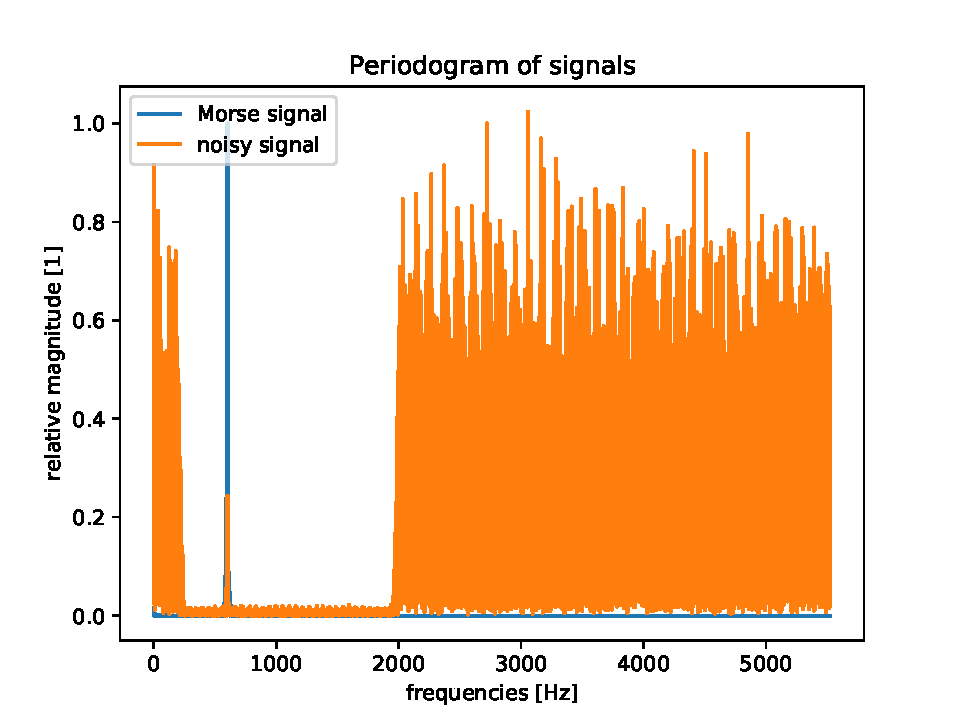
\includegraphics[]{esda_eksamen_init_sp.pdf}
	\caption{Periodogram av støyete og morse signalet}
\centering
\label{fig:init_sp}
\end{figure}

Etter som signalet kun har en frekvens ville et ideelt filter hatt en uendelig $Q$-faktor og kun tatt opp $f_0=600\si{\hertz}$, et slikt filter finnes naturligvis ikke. Vi kan derimot designe et tilstrekkelig bra filter med Delyiannis - Friend topologien vi diskuterte i seksjon \ref{sec:teori}. Av design parametrene $H_0=10$, $Q=6$ og naturligvis $f_0=600\si{\hertz}$ fungerte tilstrekkelig. Videre bestemte vi $R_3=200\si{\kilo\ohm}$ for å holde motstands verdiene rimelige. Vi har nå 3 likninger med 3 frihetsgrader, dermed kan de resterende komponentvediene bestemmes entydig. Komponent vediene som ble brukt er listet opp i tabell \ref{tab:comp_vals}. 


\begin{table}[]
    \centering
    \begin{tabular}{c|c}
      $R_1$   & $10\si{\kilo\ohm}$ \\
       $R_2$  & $1.6\si{\kilo\ohm}$\\
       $R_3$ & $200\si{\kilo\ohm}$\\
       $C$ & $16\si{\nano\farad}$\\
    \end{tabular}
    \caption{Komponent verdier}
    \label{tab:comp_vals}
\end{table}

Dette filteret er designet med relativt høy forsterking, dette gjør at kretsen vil forsterke frem selv svake signaler. For å oppnå en tilstrekkelig støydemping ble hele systemet implementert som en kaskade av 2 like filter som vist i figur \ref{fig:cascada filters}. Dermed får vi en stor forsterking ved resonans frekvensen $f_0$ som vi kan se i figur \ref{fig:bode}. 


%%%%%%%%%%%%%%%%%%%%%%%5
\begin{figure}
\centering
	\includegraphics[]{esda_eksamen_bode_data.pdf}
	\caption{bode plot for filteret}
\centering
\label{fig:bode}
\end{figure}
%%%%%%%%%55
I figurene \ref{fig:filtered_spectrogram} og \ref{fig:unfiltered_spectrogram} kan vi se at systemet filtererer ut signalet på $600\si{\hertz}$. 

\begin{figure}
\centering
	\includegraphics[]{esda_eksamen_filtered_spectrogram.pdf}
	\caption{Filtrert spectrogram}
\centering
\label{fig:filtered_spectrogram}
\end{figure}

\begin{figure}
\centering
	\includegraphics[]{esda_eksamen_unfiltered_spectrogram.pdf}
	\caption{Ufiltrert spectrogram}
\centering
\label{fig:unfiltered_spectrogram}
\end{figure}

I test implementasjonen, som avbildet i figur \ref{fig:pic} fikk vi problemer med klipping da signalet ble forsterket ut av verdiområdet som i vårt tilfelle var $\pm5V$. Dette ble løst ved å redusere amplituden på inngang signalet til $5mV$, da vil output signalet sendes ut med amplitude $5V$ ved $f_0$. Klippe problemet kunne og ha blitt løst ved å øke $V_cc$ for å tillate sterkere signaler. Vi kan ikke si noe om hvor svake signaler proffesoren jobbet med, vårt system fungerer for svake signaler, men dersom professoren komuniserte med bruk av kraftigere signaler ville han ha designet om filteret for å ha mindre forsterking. 



\section{Konklusjon}
\label{sec:konklusjon}
Test resultatene våre viser at det er meget sannsynlig at professoren kunne ha utført denne signalbehandlingsopperasjonen. Vårt system virker på svake signaler men det er relativt lett å designe om til et system som  kan motta krafigere signaler.
%Bibliografi: Legg til flere elementer ved å legge til flere \bibitem:--------
\phantomsection
\addcontentsline{toc}{section}{Referanser}
\begin{thebibliography}{99}

\bibitem{}
Per Thomas Martin Tybell, \textit{vedlegg 1}, NTNU, 2020



\end{thebibliography}




\end{document}